\section{Quadratic Splines}

A \textit{quadratic spline} is a set of piecewise quadratic functions which intersect all points in a dataset. There are three conditions that mathematically govern these functions. The first condition is that the functions must be \textit{continuous}. The second condition is that the functions must be \textit{smooth}, meaning that the derivatives are continous.

There are $3n$ unknowns, where $n$ is the number of data points in the dataset. This is because there is an $a_i$, $b_i$, and $c_i$, for each $i$ data point. We will look at a particular example with 4 points (shown in table \ref{tab:dataset}), and three connecting splines.

\begin{table}[H]
\begin{center}
\caption{Example dataset for quadratic spline}
\label{tab:dataset}
  \begin{tabular}{|c|c|c|c|c|}
    \hline
    $x$ & $x_0$ & $x_1$ & $x_2$ & $x_3$\\ \hline
    $y$ & $f(x_0)$ & $f(x_1)$ & $f(x_2)$ & $f(x_3)$\\
    \hline
  \end{tabular}
\end{center}
\end{table}

\begin{figure}[H]
\begin{center}
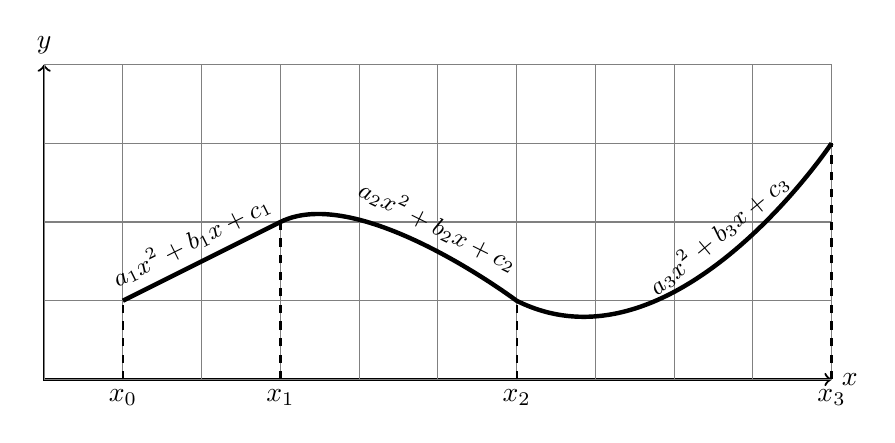
\begin{tikzpicture}
% Draw axes
\draw [<->,thick]
        (0,4) node (yaxis) [above] {$y$} |-
        (10,0) node (xaxis) [right] {$x$};
        
% Draw grid
\draw[gray, step=1cm] (0,0) grid (10,4);

% Draw path through points
        \draw [ultra thick]
        (1,1) -- 
        node[midway,above,sloped]
        {\small $a_1x^2+b_1x+c_1$}
        (3,2) .. controls (4,2.5) and (6,1) ..
        node[midway,above,sloped]
        {\small $a_2x^2+b_2x+c_2$}
        (6,1) .. controls (8,0) and (10,3) ..
        node[above,sloped]
        {\small $a_3x^2+b_3x+c_3$}
        (10,3);


% write x_0, x_1...
\draw[thick,dashed]
        (1,0) 
        node[below]{$x_0$} -- 
        (1,1);
\draw[thick,dashed]
        (3,0) 
        node[below]{$x_1$} -- 
        (3,2);
\draw[thick,dashed]
        (6,0) 
        node[below]{$x_2$} -- 
        (6,1);
\draw[thick,dashed]
        (10,0)
        node[below]{$x_3$} -- 
        (10,3);

% Draw points
\poi{1,1}
\poi{3,2}
\poi{6,1}
\poi{10,3}

\end{tikzpicture}
\caption{Example dataset plot with splines}
\label{fig:spline}
\end{center}
\end{figure}

\subsection{Continuous Functions}
The spline equations should be continuous and go through all the points in the dataset. This means that the 

\begin{align}
f(x)
=
\begin{cases}
a_1x^2 + b_1x + c_1 & x_0 < x < x_1\\
a_2x^2 + b_2x + c_2 & x_1 < x < x_2\\
a_3x^2 + b_3x + c_3 & x_2 < x < x_3\\
\end{cases}
\end{align}

The first spline equation must be equal at the start of the interval, $x_1$, to the value of dataset $f(x_0)$. As an equation this is:

\begin{align}
f(x_0) = a_1x_0^2 + b_1x_0 + c_1
\end{align}

At the point, $x_1$, the first spline equation must be equal to the output value from the dataset, $f(x_1)$. The second equation must \textit{also} be equal to this. Therefore this generates two additional equations:

\begin{align}
f(x_1) = a_1x_1^2 + b_1x_1 + c_1 \\
f(x_1) = a_2x_1^2 + b_2x_1 + c_2
\end{align}

At the second data point, $x_2$, the second and thrid spline must be equal to $f(x_2)$. This generates two additional equation.

\begin{align}
f(x_2) = a_2x_2^2 + b_2x_2 + c_2 \\
f(x_2) = a_3x_2^2 + b_3x_2 + c_3
\end{align}

Finally, the last spline must go through the last point, generating one more continuity equation:

\begin{align}
f(x_3) = a_3x_3^2 + b_3x_3 + c_3
\end{align}
%4 6 2*(4-1)
%5 8 2*(5-1)

This results in $6$ equations total leaving $3$ more unknowns that must be found. To generalize this pattern: for every $n$ points the continuity condition generates $2(n-1)$ equations.

\subsection{Smooth Functions}

Next, take the derivative of the three spline equations:

\begin{align}
	f'(x)=
\begin{cases}
	2a_1x+b_1\\ 
	2a_2x+b_2\\ 
	2a_3x+b_3 
\end{cases}
\end{align}

We know that the derivatives of the interior points must be continuous. We take the first two derivatives, evaluate them at the point $x_1$, and set them equal to each other. The same is done for spline 2 and 3. This results in two additional equations (\ref{Eq:der1}, \ref{Eq:der2}).

\begin{align}
	2a_1x_1+b_1 &= 2a_2x_1+b_2 \label{Eq:der1}\\
	2a_2x_2+b_2 &=2a_3x_2+b_3 \label{Eq:der2}
\end{align}

Rewriting the equations to move all the variables to the left side:

\begin{align}
	2a_1x_1+b_1 - 2a_2x_1-b_2 &=0\\
	2a_2x_2+b_2 - 2a_3x_2-b_3 &=0
\end{align}

To generalize this pattern, the smooth function condition produces $(n-2)$ equations. We now have 9 unknowns but only 8 equations. The last equation is the decision that the first spline will be linear. This is written in equation \ref{Eq:a10}

\begin{align}
	a_1=0
	\label{Eq:a10}
\end{align}

% stretch matrix vertically.
% This will be undone after the matrix
\renewcommand\arraystretch{1.3}

\begin{equation}
\begin{blockarray}{cccccccccc}
%% First are continuity condition
    & a_1 & b_1 & c_1 & a_2 & b_2 & c_2 & a_3 & b_3 & c_3 \\
  \begin{block}{c[ccccccccc]}
	f_1 & x_0^2 & x_0 & 0 & 0 & 0 & 0 & 0 & 0 & 0 \\
	f_2 & x_1^2 & x_1 & 0 & 0 & 0 & 0 & 0 & 0 & 0 \\
	f_3 & 0 & 0 & 0 & x_1^2 & x_1 & 0 & 0 & 0 & 0 \\
	f_4 & 0 & 0 & 0 & x_2^2 & x_2 & 0 & 0 & 0 & 0 \\
	f_5 & 0 & 0 & 0 & 0 & 0 & 0 & x_2^2 & x_2 & 0 \\
	f_6 & 0 & 0 & 0 & 0 & 0 & 0 & x_3^2 & x_3 & 0 \\
%% Next are smooth function equations
  \end{block}
\end{blockarray}
\end{equation}
\renewcommand\arraystretch{1}

\section{Coding Quadratic Splines}


\begin{pseudocode}
\item Define dataset or take dataset as input if programmed as a stand alone function
\item Initialize $\vec{A}$ as a matrix of zeros $(3n,3n)$
\item Initialize $\vec{b}$ as a matrix of zeros $(30,1)$
\item Loop through number of points and use continuous function information

\begin{enumerate}
\item Set values for first equation
\end{enumerate}

\item Loop through number of points and use continuous derivatives information
\begin{enumerate}
\item Use interior points
\end{enumerate}

\item Solve the system of equations for the constants
\item Plot and output values
\begin{enumerate}
	\item Plot the piecewise quadratic function \textit{only} in the intervals where they are valid.
	\item Scatter plot points
	\item Plot query point, if any
\end{enumerate}

\end{pseudocode}